\subsection{System level}
	The following graph is our system level state chart, which contains all our class level state charts. It shows how all classes interact.

	\includegraphics[width=\linewidth]{statecharts/system.pdf}

\subsection{Class level}
	\subsubsection{Board}
	First the board is initialized, then the board has to initialize the controller. After that, the board goes to the NOP state from which it can answer requests from robots to move; it can also notify robots if they receive a hint, win the game or get moved by the board. Every time the board has done something, it returns to the NOP state, except when a robot has reached it's hometile. In this case, the board has to terminate other classes via the reset() function. After the game is over, the board can either terminate or go back to the initialized state to start a new game.
	
	\includegraphics[width=\linewidth]{statecharts/board.pdf}

	\subsubsection{Controller}
	The controller initializes in two phases: the first phase is the preInitialize() function and the second phase is the postInitialize() function. After the postInitialize, the class is in the NOP state. From this state, all events take place. The controller can pass on the requestSnapshot() call from the board to the viewer class. The controller also sends move requests to the board. However, the board has to answer the request, so the controller goes to the MoveRequestProcessed state. During this state, it will wait for the board to answer. After the move request has been answered and it was successful, two tiles are switched and. Even more, when robots have been moved, these robots receive a notifyAutoMovement(). After the tiles have been switched, the controller returns to the NOP state. If a robot requests a move and the board concludes that the robot has reached its hometile, the controller terminates because the game is over.

	\includegraphics[width=\linewidth]{statecharts/controller.pdf}

	\subsubsection{Viewer}
	After being initialized, the viewer goes to the NOP state. It checks the board for changes via a Controller.requestBoardStatus() call every now and then. If the board has been changed, the Viewer receives a notifyStateChange() from the Controller. Hereafter, the function updateView() is called to make the changes visible. The viewer is removed when the game is over, but it may also decide to remove itself.
	
	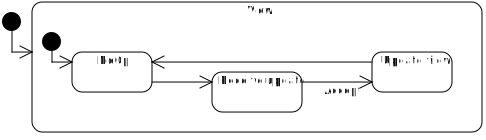
\includegraphics[width=\linewidth]{statecharts/view.pdf}

	\subsubsection{Robot}
	The robot class receives an initialize(). The robot begins on a randomly picked spot, which can be a normal tile, a hint tile or a conveyer tile. The robot receives a notifyAutomovement() every time it gets moved. This can happen in two ways: the robot steps on a conveyor belt or the robot gets moved via a tiles witch. Whenever a robot is on a tile, it can request a move. The result of this request is either SUCCESS, FAILED or WIN. If a move request is successful, the move is done. If a move request is a failure, the move is rejected, since the desired path of the move is blocked. If the robot ends up on its home tile, the move request results in a WIN and the game ends. When another robot wins, this robot gets a terminate request from the controller and the game is over. The robot can also encounter hint tiles which point the robot to the location of its home tile.
	
	\includegraphics[width=\linewidth]{statecharts/robot.pdf}
	

	
